% !TeX root = Protokoll.tex
\subsection{Versuchsaufbau}
\begin{figure}
	\centering
	\begin{tikzpicture}
			
			\node [draw=white, anchor=south west] (label) at (0,0) {
				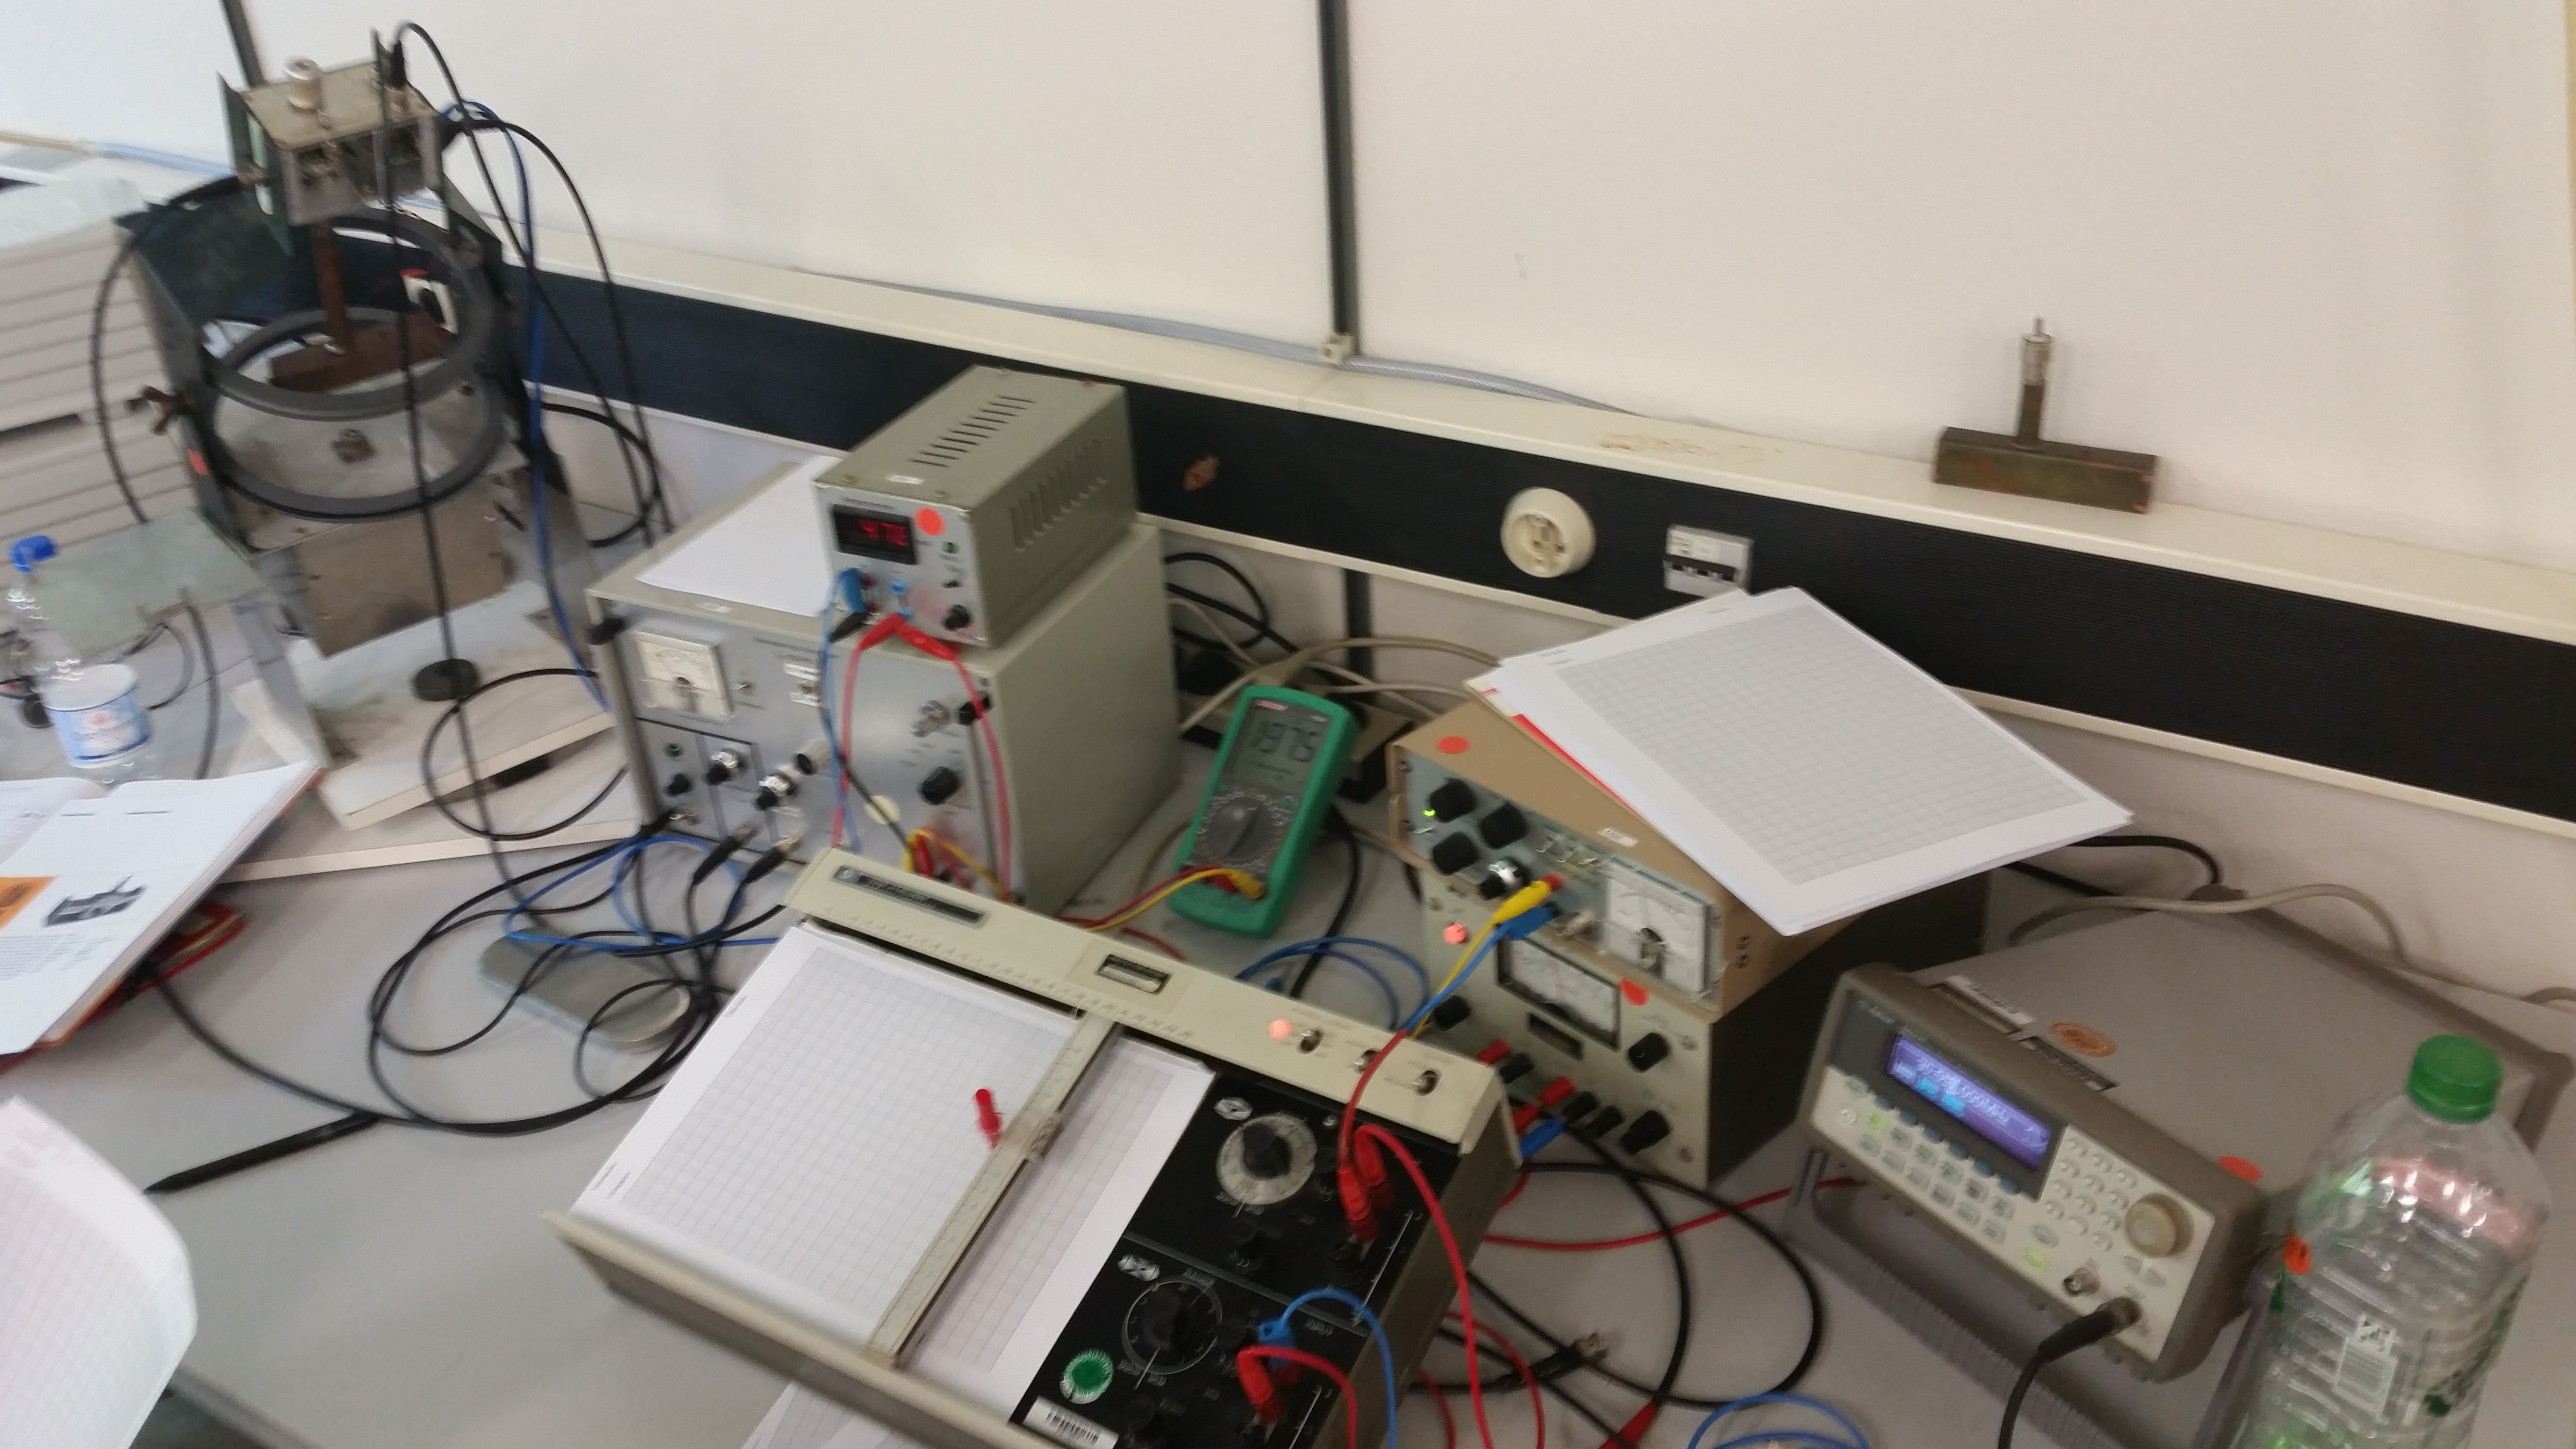
\includegraphics[width=1.0\textwidth]{../Grafiken/Aufbau.jpg}};
%			\draw[step=.5cm,draw=gray] (0.0,0.0) grid (\textwidth,\textwidth - 180);
%			\foreach \x in {0,1,...,16}
%				\filldraw [fill=green] (\x,0) node[below] {\x};
%			\foreach \y in {0,1,...,10}
%				\filldraw [fill=green] (0,\y) node[left] {\y};
				
			\draw [very thick] (2.0,8.5) -- (1.0,8.5);
			\node [draw=black,shape=circle,fill=lightgray] (1.) at (1.0,8.5) {1};
			\draw [very thick] (3.0,7.5) -- (4.0,7.5);
			\node [draw=black,shape=circle,fill=lightgray] (1.) at (4.0,7.5) {2};
			\draw [very thick] (2.25,6.85) -- (1.0,6.85);
			\node [draw=black,shape=circle,fill=lightgray] (1.) at (1.0,7.0) {3};
			\draw [very thick] (5.0,5.5) -- (5.0,6.5);
			\node [draw=black,shape=circle,fill=lightgray] (1.) at (5.0,6.5) {4};
			\draw [very thick] (6.0,6.5) -- (6.0,7.5);
			\node [draw=black,shape=circle,fill=lightgray] (1.) at (6.0,7.5) {5};
			\draw [very thick] (8.0,4.5) -- (8.0,5.5);
			\node [draw=black,shape=circle,fill=lightgray] (1.) at (8.0,5.5) {6};
			\draw [very thick] (7.0,3.0) -- (7.0,4.0);
			\node [draw=black,shape=circle,fill=lightgray] (1.) at (7.0,4.0) {7};
			\draw [very thick] (9.5,4.5) -- (9.5,5.5);
			\node [draw=black,shape=circle,fill=lightgray] (1.) at (9.5,5.5) {8};
			\draw [very thick] (10.5,2.) -- (10.5,1.);
			\node [draw=black,shape=circle,fill=lightgray] (1.) at (10.5,1.) {9};
			\draw [very thick] (13,2.5) -- (13.,3.5);
			\node [draw=black,shape=circle,fill=lightgray] (1.) at (13.,3.5) {10};						

		\end{tikzpicture}
			\caption{Der verwendete Versuchsaufbau zur Durchführung von ESR-Messung}\label{fig:Aufbau}
\end{figure}

In \cref{fig:Aufbau} ist der Versuchsaufbau dargestellt.
Oben links ist die Probe (1) zusehen die sich innerhalb einer Helmholtz-Spule befindet (2), dabei wurde die Helmholtz-Spule so ausgerichtet das sie parallel beziehungsweise anti parallel zum Erdmagnetfeld ist. 
Um die Probe ist noch eine kleinere Spule die an eine Brückenschaltung (3) angeschlossen ist, diese Spule wird durch einen Hochfrequenz-Generator betrieben (9), in der Brückenschaltung ist noch ein Empfänger eingebaut mithilfe das Signal von Störungen getrennt werden kann.
Rechts neben der Brückenschaltung ist ein Multimeter (5) mit dem die Spannung der Brückenschaltung gemessen werden kann.
Rechts davon ist der Rampengenerator (7) zusehen mit dem die Helmholtz-Spule betrieben wird.
Im Vordergrund ist ein XY-Schreiber (6) zu sehen wo die Spannung der Brückenschaltung und des Rampengenerator angelegt werden.
Die Stromstärke an der Helmhotz-Spule kann mit einem Ampere Meter gemessen werden (4).
\subsection{Messverfahren}
An der Brückenschaltung können die Frequenzen $\nu_\text{Osz}$ und $\nu_\text{ZF}$ eingestellt werden, mit diesen beiden Frequenzen kann das Störsignal verringert werden und das Signal der Elektronen $\nu_e$ ausgefiltert werden. Dabei gilt
\begin{align}
	\nu_e=\nu_\text{ZF}+\nu_\text{Osz},
\end{align}
dies ist die Frequenz die am Hochfrequenz-Generator eingestellt werden sollte.
Bei abgestellten Magnetfeld der Helmholtz-Spule wird eine die minimale Brückenspannung eingestellt, indem der Kondensator $C$ und der Wiederstand $R$, der Brückenschaltung verstellt werden, dann wird das Signal mithilfe des Verstärkers auf ein Maximum verstärkt.\\
Nun wird der mithilfe des Rampengenerators eine Sägezahnspannung an die Helmholtz-Spule angelegt.
Im Spannungsverlauf der Brückenschaltung sollte ein globales Maximum oder ein globales Minimum zu sehen sein (\cref{fig:Resonanz}). 
Kann sowohl ein Maxima als auch ein Minimum zu erkennt werden, liegt eine Überlagerung der beiden Kurven vor.
Dies Geschieht dadurch das $C$ an der Brückenschaltung verstimmt ist.
 Dies kann durch feines verstellen der Brücke ausgeglichen werden.
\begin{figure}[h!]
\centering
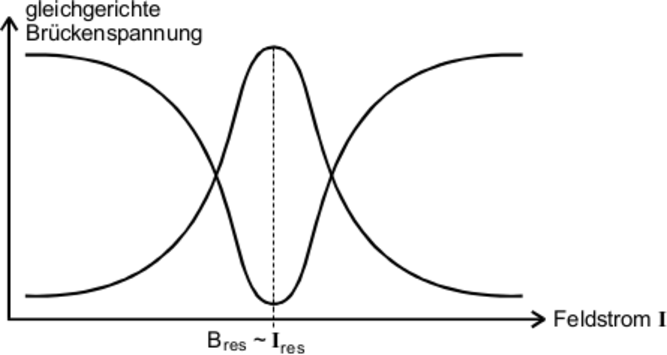
\includegraphics[width=\textwidth]{../Grafiken/Resonanz.pdf}
\caption{Darstellung der des Bildes, dass auf dem XY-Schreiber zu sehen sein sollte.\cite{V28}}\label{fig:Resonanz}
\end{figure}
Um das Bild des XY-Schreibers auswerten zu können wird die Größe der Stromstärke in einem bestimmten Bereich benötigt.
Die magnetische Feldstärke der Helmholtz-Spule ergibt sich dabei aus dem Strom $I$ durch die Spule, der Windungszahl $N$ und
dem Spulenradius $R$ nach,
\begin{empheq}{equation}
	B(I) = \dfrac{8\cdot \mu_0}{\sqrt{125}} \cdot \dfrac{I\cdot N}{R}.
	\label{eq:helmholtz}
\end{empheq}
